\section*{Problem 2.1 - Path Following with Crab angle Compensation}
\subsection*{Problem 2.1}
We implement a LOS guidance system using lookahead-based steering. The principle of this method is to move from one waypoint to the next by finding the LOS vector, and setting the desired course to move the vessel along this vector. Using the lookahead-based steering method, we separate the desired course a sum of the path-tangential angle and the velocity-path relative angle. The path-tangential angle can easily be found as the angle between the two waypoints, while the velocity-path relative angle can be found as using arctan of minus the cross-track error, divided by the distance between where the cross-track error and the LOS vector intercepts the line between the waypoints. 

We ended up choosing the same radius for all waypoints, set to be slightly larger than double the length of the vessel. Furthermore, we also limited delta to be between 0 and R. 

\subsection*{Problem 2.2}
See \figref{fig:path_2_2} for the path of the vessel, and \figref{fig:cross_track_error2_2} for the cross-track error. Note that the variable for stopping the simulation has been reduced, so that it's easier to see the valid track between the waypoints. 

\begin{figure}[ht]
	\begin{subfigure}[b]{0.4\textwidth}
		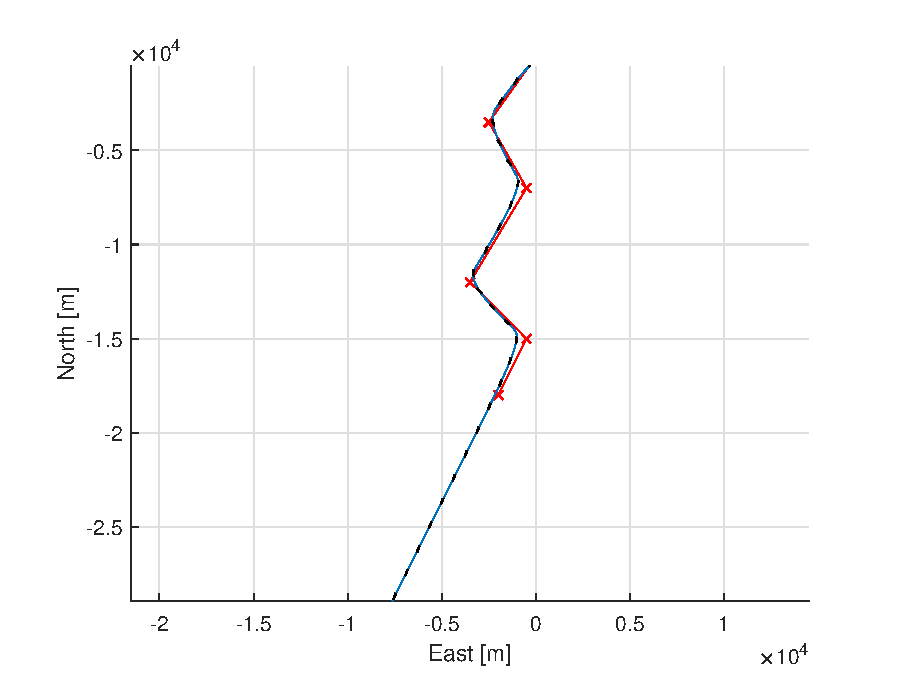
\includegraphics[width=\textwidth]{path_2_2}
		\caption{Path and waypoints}
		\label{fig:path_2_2}
	\end{subfigure}%
        ~
	\begin{subfigure}[b]{0.4\textwidth}
		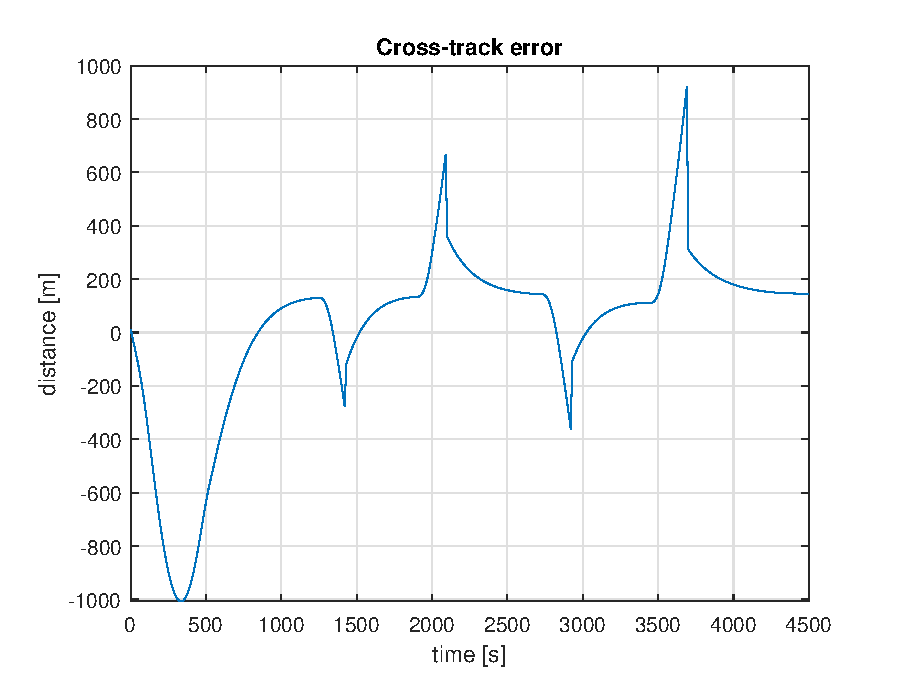
\includegraphics[width=\textwidth]{cross_track_error2_2}
		\caption{Cross-track error}
		\label{fig:cross_track_error2_2}
	\end{subfigure}
	\label{fig:task2_2}
\end{figure}

\subsection*{Problem 2.3}
The path-following is not really working as expected, as the ship doesn't seem to align properly with the path between the waypoints. This can be illustrated in \figref{fig:cross_track_error2_2}, where the cross-track error doesn't converge to zero, as it should, but rather to some other value. 

\section*{Problem 2.2 - Path Following with Crab angle Compensation}
\subsection*{Problem 2.4}
See \figref{fig:angles2_4}. We may note that the heading follows the desired course closely, as we would expect as the desired heading is set to be equivalent to desired course. However, the real course is then off by the crab angle from the heading. This should be expected considering the implementation, but is obviously not what we want. 

\begin{figure}[ht]
	\centering
	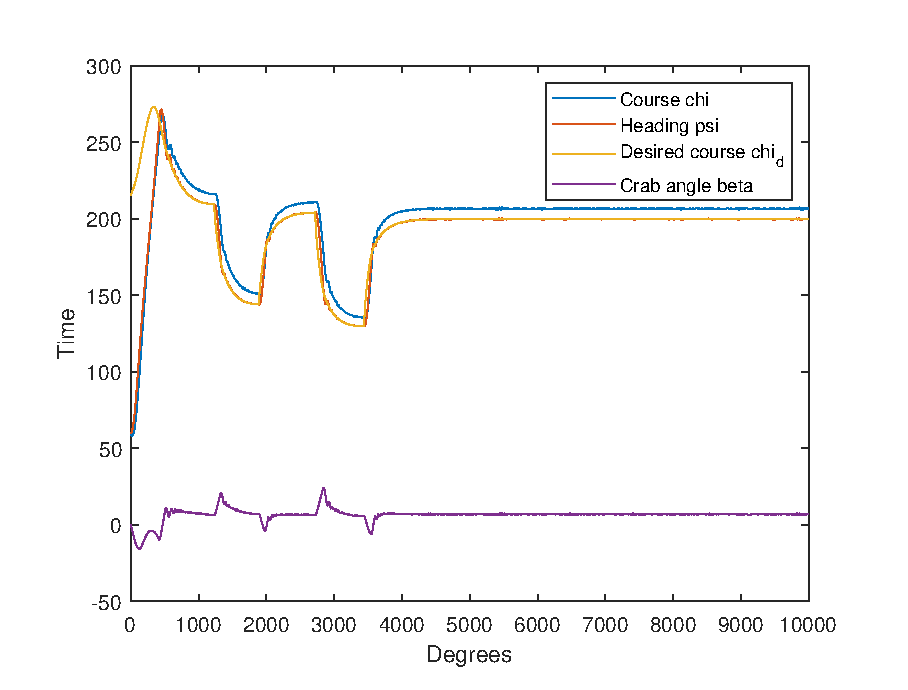
\includegraphics[width=\textwidth]{angles2_4}
	\caption{The angles generated by task 2.2}
	\label{fig:angles2_4}
\end{figure}

\subsection*{Problem 2.5}
The transforms were computed using the following equations: 
\begin{align*}
	\beta_c &= atan2(v, u) \\
	psi_d &= chi_d - beta_c \\
	u_d &= \sqrt{U_d^2 - v^2}
\end{align*}

Of course this would assume that $v$ is smaller than $U_d$, but this assumption is fair in this case. 

\subsection*{Problem 2.6}
Observing \figref{fig:angles2_6}, the course seems to better follow the desired course. This also leads to a cross-track error, see \figref{fig:cross_track_error2_6} which converges to zero, rather than some offset, as we now compensate for crab angle. In \figref{fig:path_2_6} we can see how the boat now follows the path. 

The oscillations in the system were undesirable, but we couldn't really find a way to suppress them. When observing $\delta_c$, it is often saturated, which seems to cause the oscillations. This may be because of the simplified model used to generate the heading controller. 

\begin{figure}[ht]
	\begin{subfigure}[b]{0.4\textwidth}
		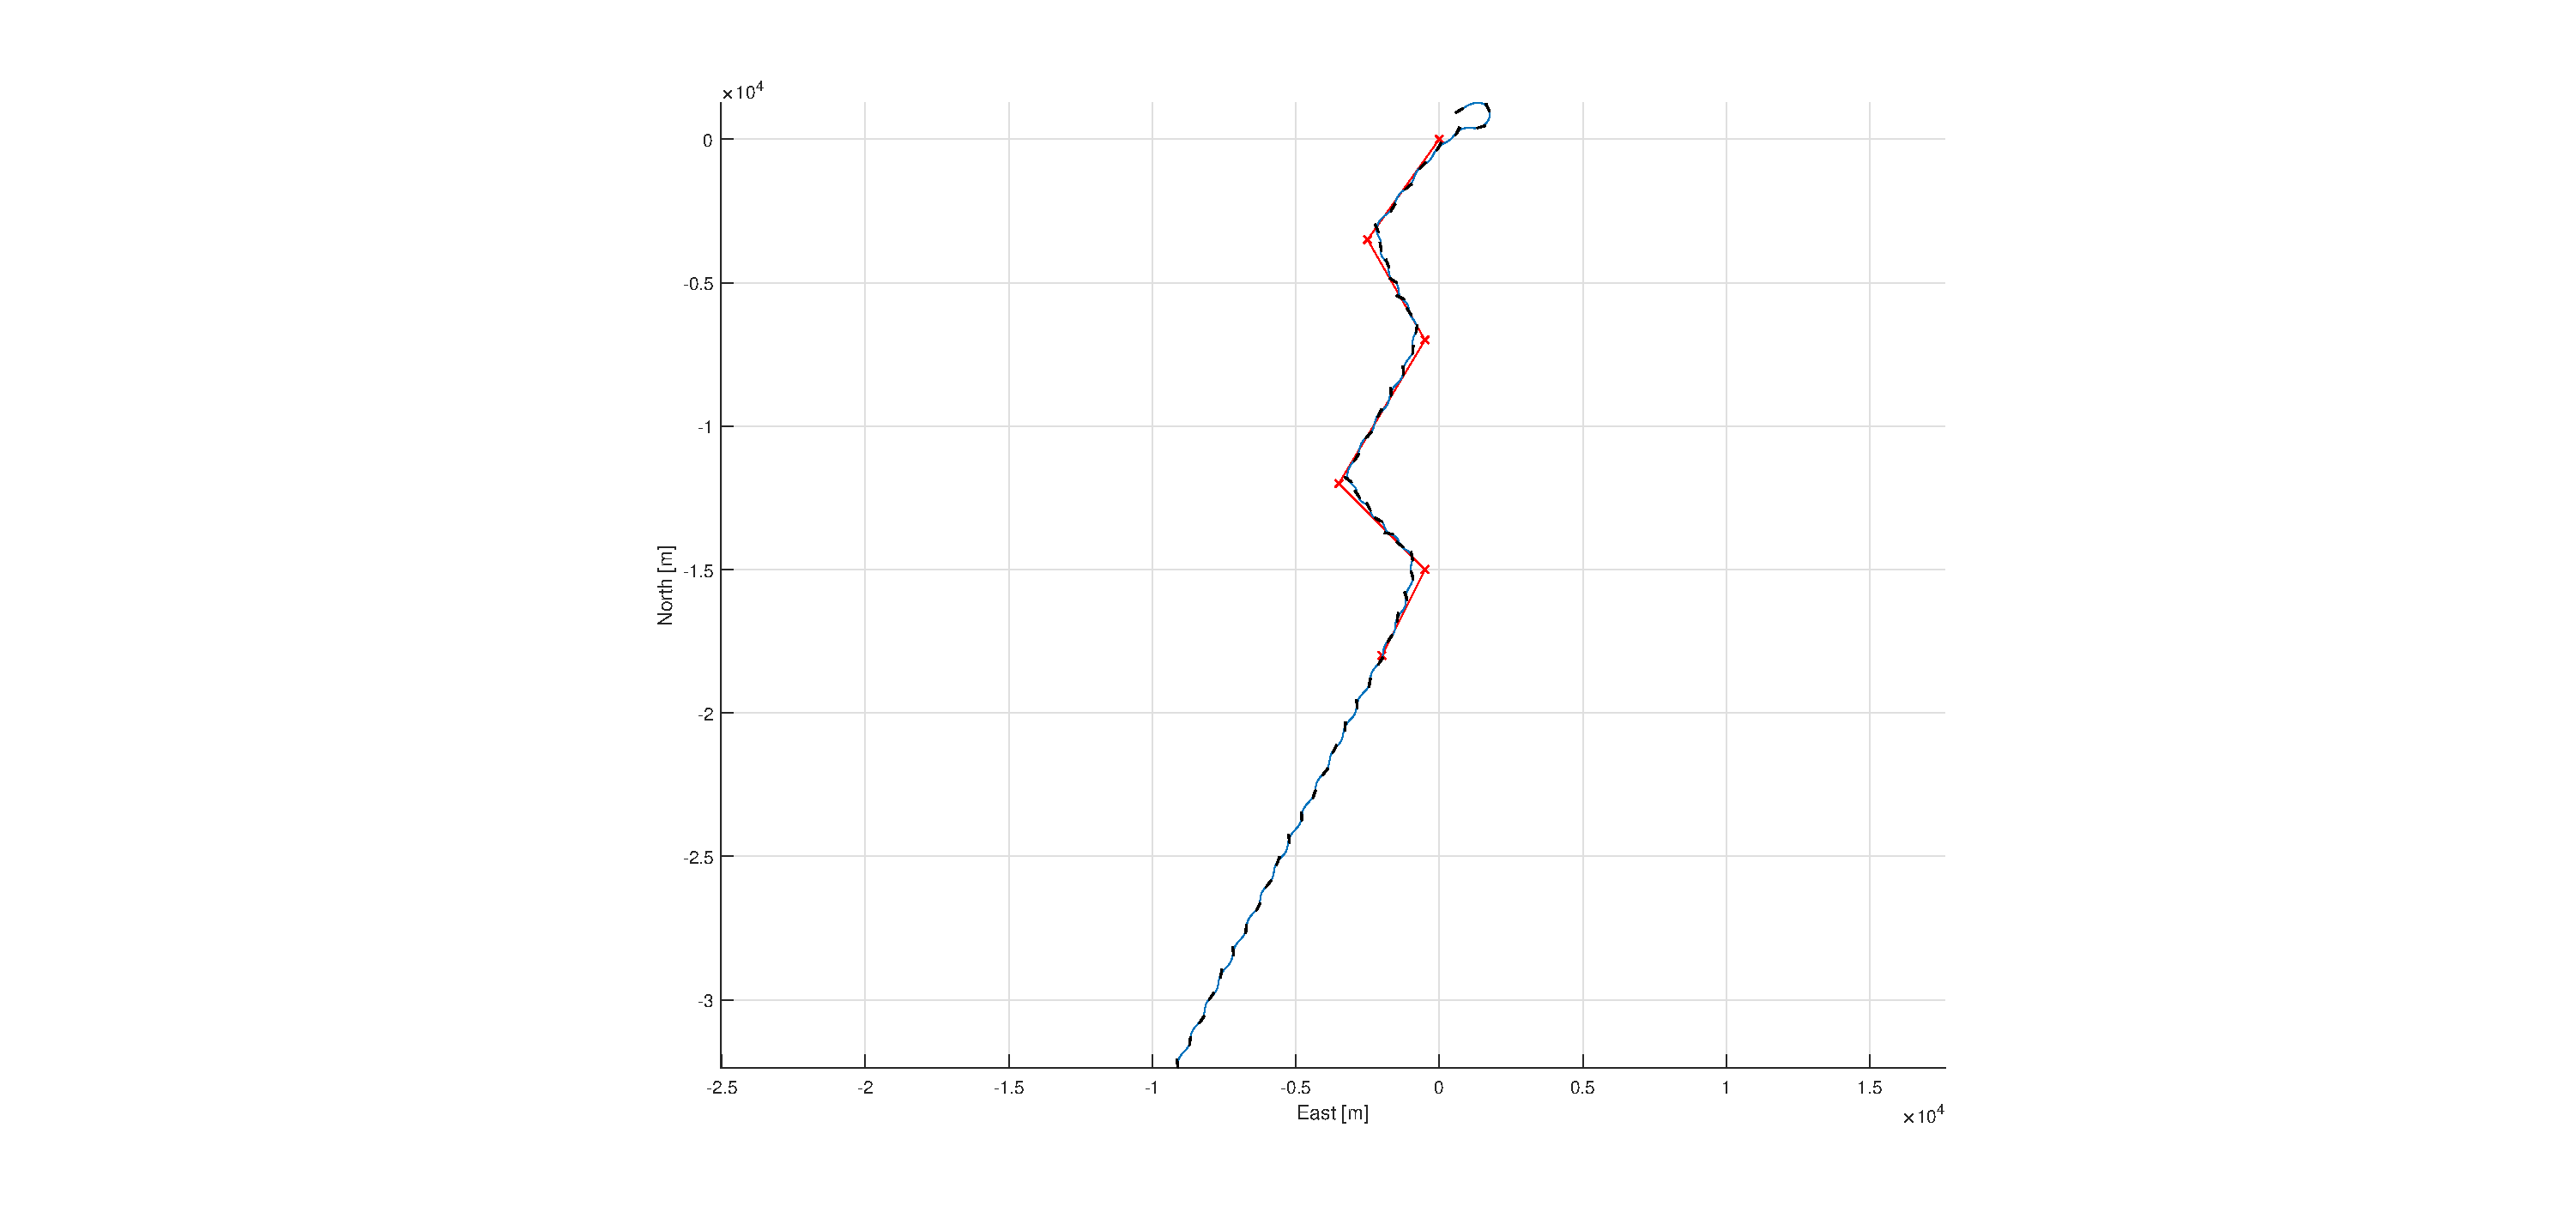
\includegraphics[width=\textwidth]{path_2_6}
		\caption{Path and waypoints}
		\label{fig:path_2_6}
	\end{subfigure}%
        ~
	\begin{subfigure}[b]{0.4\textwidth}
		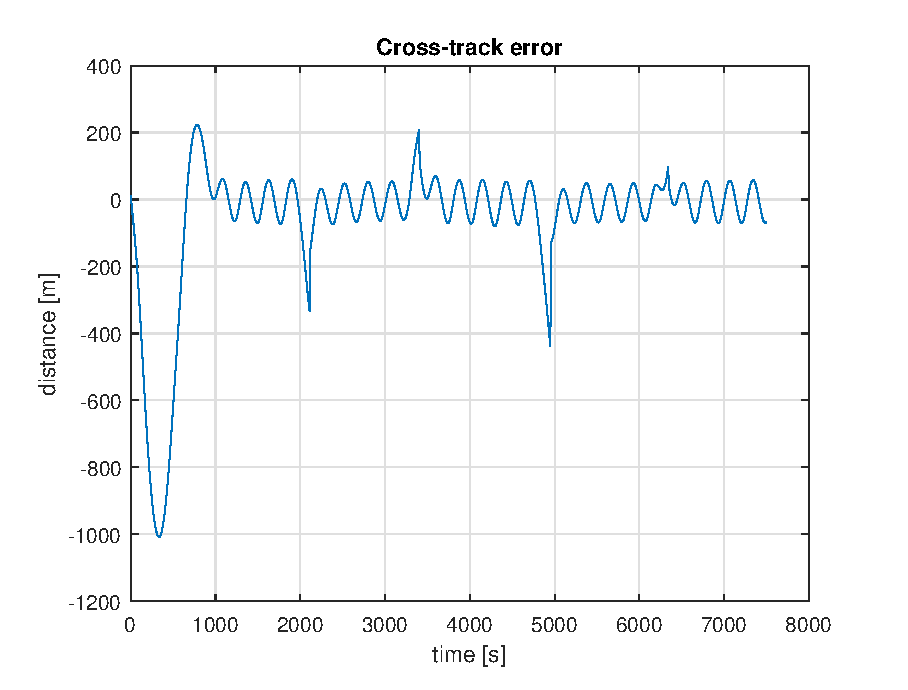
\includegraphics[width=\textwidth]{cross_track_error2_6}
		\caption{Cross-track error}
		\label{fig:cross_track_error2_6}
	\end{subfigure}
	\label{fig:task2_6}
\end{figure}

\begin{figure}[ht]
	\centering
	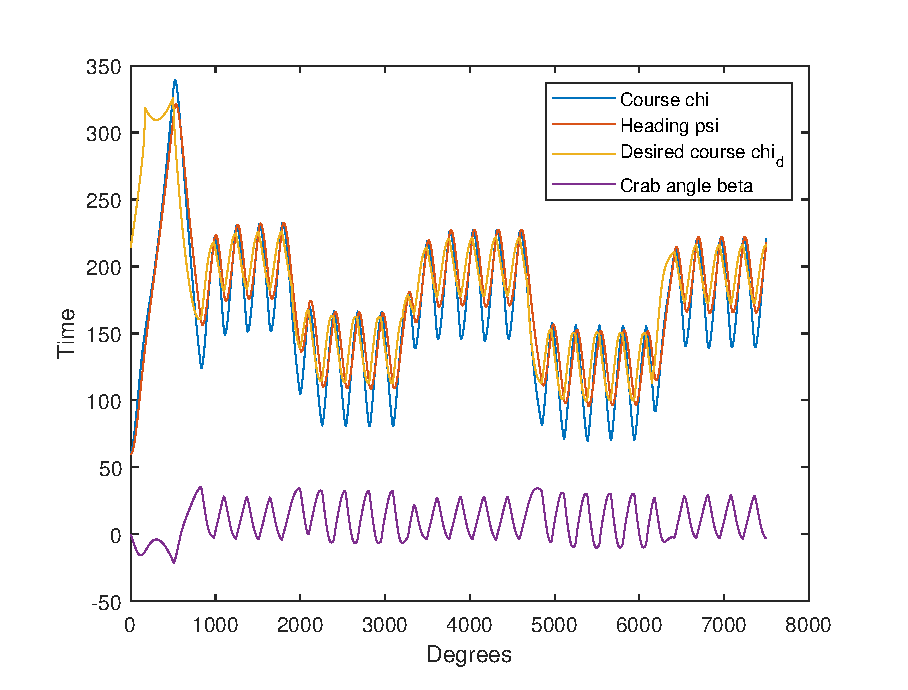
\includegraphics[width=\textwidth]{angles2_6}
	\caption{The angles generated by task 2.6}
	\label{fig:angles2_6}
\end{figure}

\section*{Problem 2.3 - Target Tracking}
\subsection*{Problem 2.7}
For this task we implemented the pure-pursuit target-tracking system. The distance to target is set to two times the boat length. 

\begin{figure}[ht]
	\begin{subfigure}[b]{0.3\textwidth}
		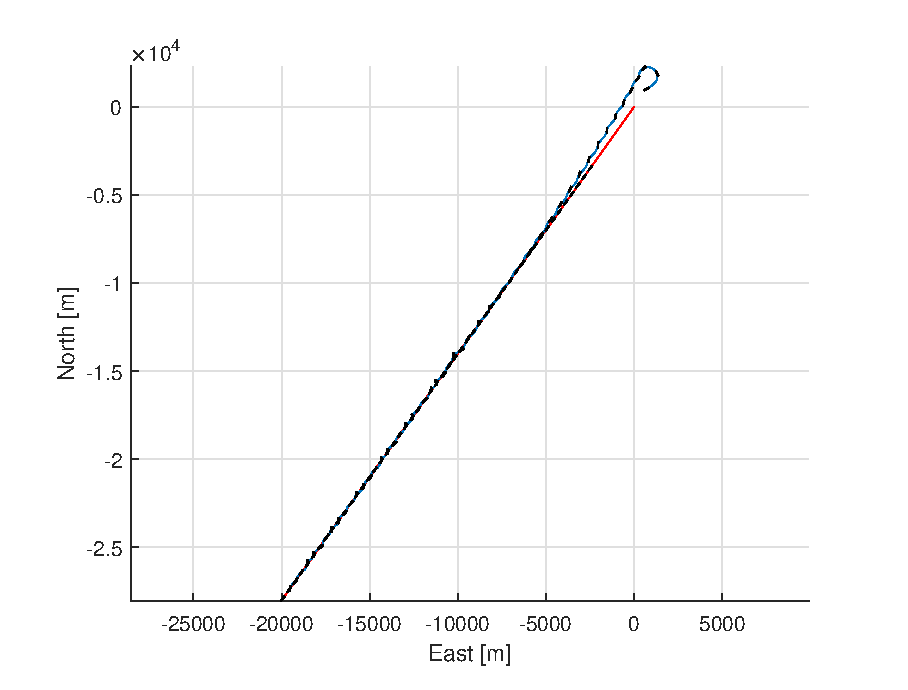
\includegraphics[width=\textwidth]{path_2_7}
		\caption{Path of vessel}
		\label{fig:path_2_6}
	\end{subfigure}%
        ~
	\begin{subfigure}[b]{0.3\textwidth}
		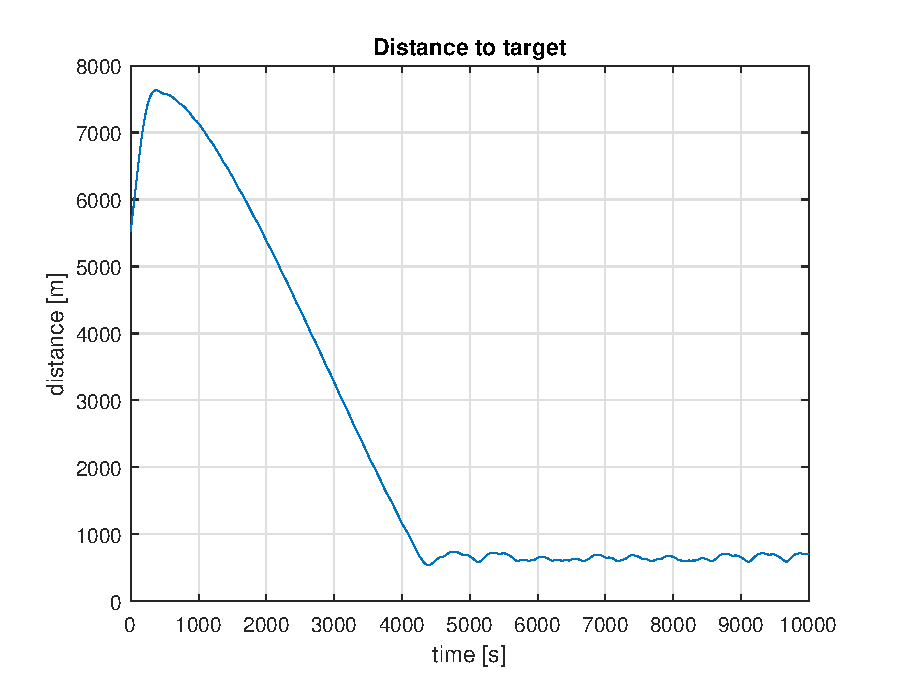
\includegraphics[width=\textwidth]{distance_to_target2_7}
		\caption{Absolute distance to target}
		\label{fig:distance_to_target2_7}
	\end{subfigure}
	\label{fig:task2_6}%
	~
	\begin{subfigure}[b]{0.3\textwidth}
		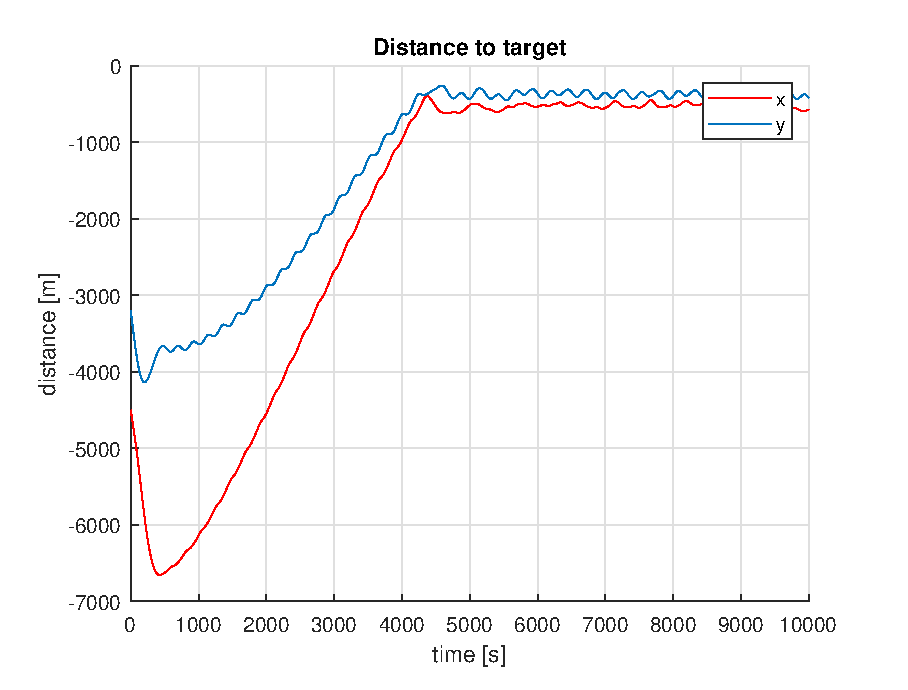
\includegraphics[width=\textwidth]{x_y_distance_to_target2_7}
		\caption{Distance to target, x and y}
		\label{fig:x_y_distance_to_target2_7}
	\end{subfigure}
	\label{fig:task2_7}
\end{figure}